% Time-stamp: <2025-03-05 16:02:11>


\documentclass[presentation,aspectratio=1610]{beamer}

%% Full theme: AnnArbor Antibes Bergen Berkeley Berlin Boadilla boxes CambridgeUS Copenhagen Darmstadt default Dresden EastLansing Frankfurt Goettingen Hannover Ilmenau JuanLesPins Luebeck Madrid Malmoe Marburg Montpellier PaloAlto Pittsburgh Rochester Singapore Szeged Warsaw
% \usetheme{Luebeck}

%% outer themes (header/footer): default infolines miniframes smoothbars sidebar split shadow tree smoothtree
% \useoutertheme[subsection=false]{smoothbars}
% \usetheme{Rochester}
 \useoutertheme{split}

%% inner theme (content): default circles rectangles rounded inmargin
\useinnertheme{rectangles}

\usecolortheme{beaver}

\input{style}



\defcolvar{n}{n}{red}
\defcolvar{alpha}{\alpha}{red}
\defcolvar{S}{S}{darkgreen}
\defcolvar{x}{x}{blue}
\defcolvar{y}{y}{blue}
\defcolvar{q}{q}{red}

\title{Symmetric Techniques for Advanced Protocols: What *are* They?}
\author[Léo Perrin]{Léo Perrin\inst{1} }

\institute{Inria, Paris}
\titlegraphic{\includegraphics[height=1.1cm]{figures/inria}}


\date{14th of March 2025}




\begin{document}

{
  \pagestyle{empty}

  \maketitle


  \begin{frame}{Trendy topics}

    \begin{itemize}
      \large
    \item [] MPC-friendly? 
    \item [] Arithmetization-Oriented?
    \item [] Verification efficiency?
    \item [] Algebraic attacks? \pause
    \item [] Symmetric crypto \textbf{for the blockchain...} \pause
    \item [] \alert{... for neural networks???}
    \end{itemize}
    \begin{center}
      The conclusion of today: \textbf{symmetric cryptography} has always had to deal with specific \textbf{implementation criteria}, but the \alert{new ones} are indeed a bit \textbf{stranger than before}.
    \end{center}
  \end{frame}
}


\tocStartsAppearingHere{}


\section{What is the Purpose of a Symmetric Primitive}

\subsection{Let's look at primitives we all know}


\begin{frame}{Let's talk!}
  \vfill

  \begin{center}
    \includegraphics[width=8cm]{./figures/simpsons}
  \end{center}
  
  \vfill
\end{frame}


\begin{frame}{Unstable Definitions}
  \begin{alertblock}{What is ``efficient'' varies}
    \begin{itemize}
    \item What are the operations that we \textbf{can} use?
    \item What are the associated \textbf{costs}? 
    \end{itemize}
    \begin{center}
      How to get the best security for a given price?
    \end{center}
  \end{alertblock}

  
  
  \begin{exampleblock}{What is ``secure'' varies}
    \begin{itemize}
    \item Should the primitive work in many context? \hfill\onslide<4>{Modularity vs. Single use}
    \item Do we care about nonce-misuse? \hfill\onslide<4>{Robustness vs. ``not our problem''}
    \end{itemize}
    \begin{center}
      How do we define the \textbf{security} that the primitive must provide?
    \end{center}
  \end{exampleblock}
\end{frame}


\subsection{A Small Cog in a Big Machine}


\begin{frame}{Web Encryption}
  \begin{center}
    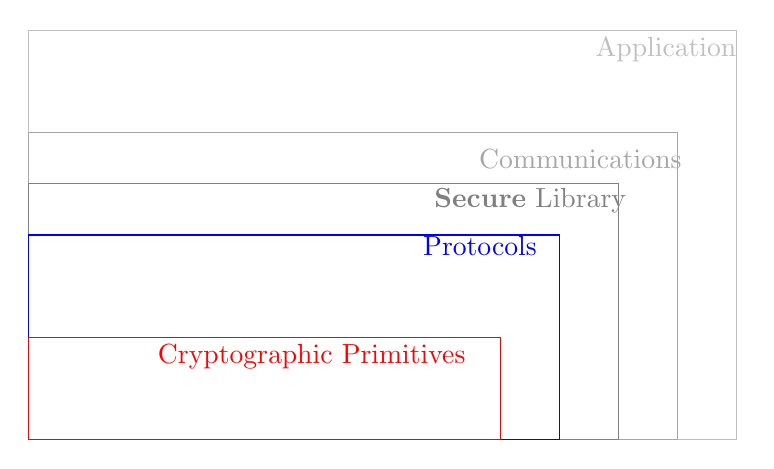
\begin{tikzpicture}[xscale=1.5,yscale=1.3]
      \draw[color=gray!50!white] (0, 0) rectangle (6, 4) node[pos=0.9,above] {Application};
      \onslide<2->{
        \draw[color=gray!70!white] (0, 0) rectangle (5.5, 3) node[pos=0.85,above] {Communications};
      }
      \onslide<3->{
        \draw[color=gray] (0, 0) rectangle (5, 2.5) node[pos=0.85,above] {\textbf{Secure} Library};
      }
      \onslide<4->{
        \draw[color=blue] (0, 0) rectangle (4.5, 2) node[pos=0.85,above] {Protocols};
      }
      \onslide<5->{
        \draw[color=red] (0, 0) rectangle (4, 1) node[pos=0.6,above] {Cryptographic Primitives};
      }
    \end{tikzpicture}

    \begin{itemize}
    \item<6-> We want \alert{software efficient} (computer and smartphone but not micro-controllers) efficient \alert{AEAD}.
    \item<7> AES-GCM; Chacha-poly1305.
    \end{itemize}
  \end{center}
\end{frame}


\begin{frame}{What Chacha looks like}
  \begin{columns}
    \hfill
    \begin{column}{0.4\textwidth}
      \begin{center}
        \includegraphics[width=4cm]{./figures/chacha}
      \end{center}
    \end{column}
    \hfill
    \begin{column}{0.4\textwidth}
      \begin{itemize}
      \item Addition ~/~ Rotation ~/~ XOR
      \item 256-bit key
      \item 512-bit state
      \end{itemize}
    \end{column}
    \hfill
  \end{columns}
\end{frame}


\begin{frame}{RAM Encryption}
  \begin{center}
    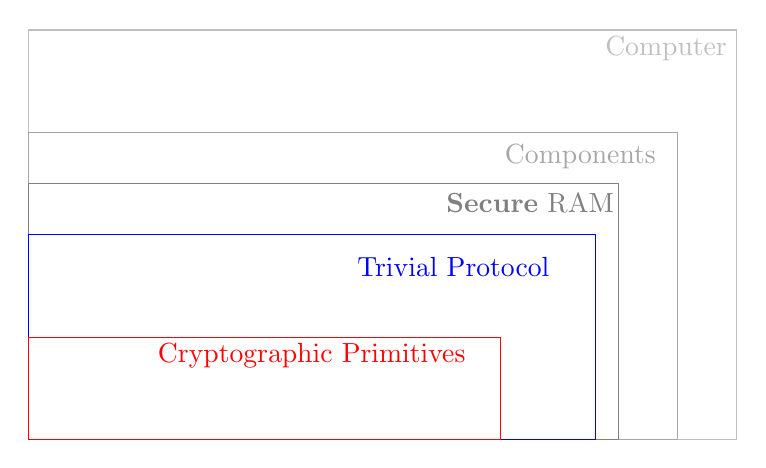
\begin{tikzpicture}[xscale=1.5,yscale=1.3]
      \draw[color=gray!50!white] (0, 0) rectangle (6, 4) node[pos=0.9,above] {Computer};
      \onslide<2->{
        \draw[color=gray!70!white] (0, 0) rectangle (5.5, 3) node[pos=0.85,above] {Components};
      }
      \onslide<3->{
        \draw[color=gray] (0, 0) rectangle (5, 2.5) node[pos=0.85,above] {\textbf{Secure} RAM};
      }
      \onslide<4->{
        \draw[color=blue] (0, 0) rectangle (4.8, 2) node[pos=0.75,above] {Trivial Protocol};
      }
      \onslide<5->{
        \draw[color=red] (0, 0) rectangle (4, 1) node[pos=0.6,above] {Cryptographic Primitives};
      }
    \end{tikzpicture}

    \begin{itemize}
    \item<6-> We want \alert{very low latency} \alert{block encryption}.
    \item<7> PRINCE? QARMA? not so clear at this stage.
    \end{itemize}
  \end{center}
\end{frame}


\begin{frame}{What PRINCE looks like}
  \begin{center}
    \includegraphics[width=12cm]{./figures/prince}

    \begin{itemize}
    \item 4-bit S-box optimized for hardware
    \item 2 different matrices
    \item FX construction
    \item ``$\alpha$-reflexion''
    \item inverse rounds used in the second half
    \end{itemize}

  \end{center}
\end{frame}


\begin{frame}{Some Constants}
  \begin{itemize}
    \setlength\itemsep{1cm}
    \large
  \item A symmetric primitive is a very \alert{small} (but crucial) cog in a
    very big machine, \pause
  \item there are many \alert{different} ``big machines'', and \pause
  \item this has a \alert{huge influence} on what the primitive looks like.
  \end{itemize}
\end{frame}


\section{``Advanced'' Protocols}

\subsection{General Introduction}

\begin{frame}{Securing Data}
  \begin{center}
    {\Large Usually, we secure \alert{data} (at rest or in transit).}
    
    \only<1>{
\includegraphics[width=9cm]{./figures/crypto}}
    \only<2>{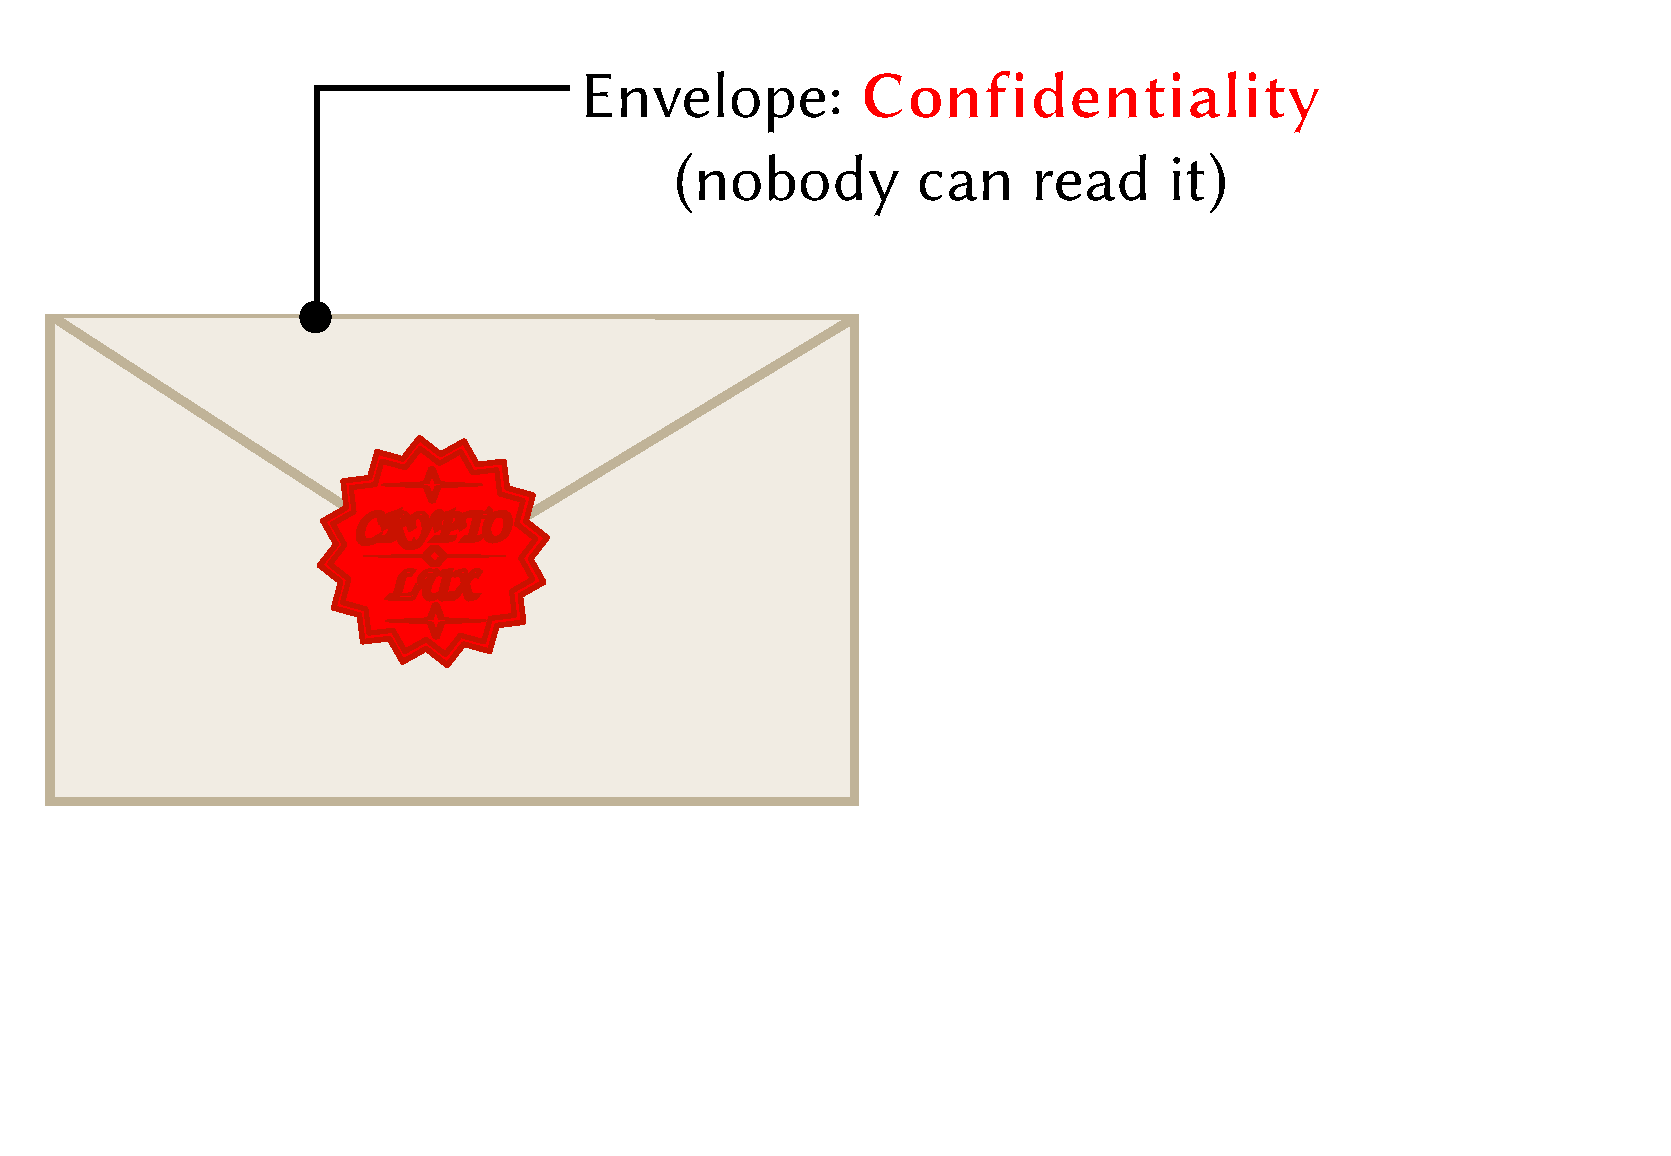
\includegraphics[width=9cm]{./figures/crypto-conf}}
    \only<3>{\includegraphics[width=9cm]{./figures/crypto-conf-int}}
    \only<4>{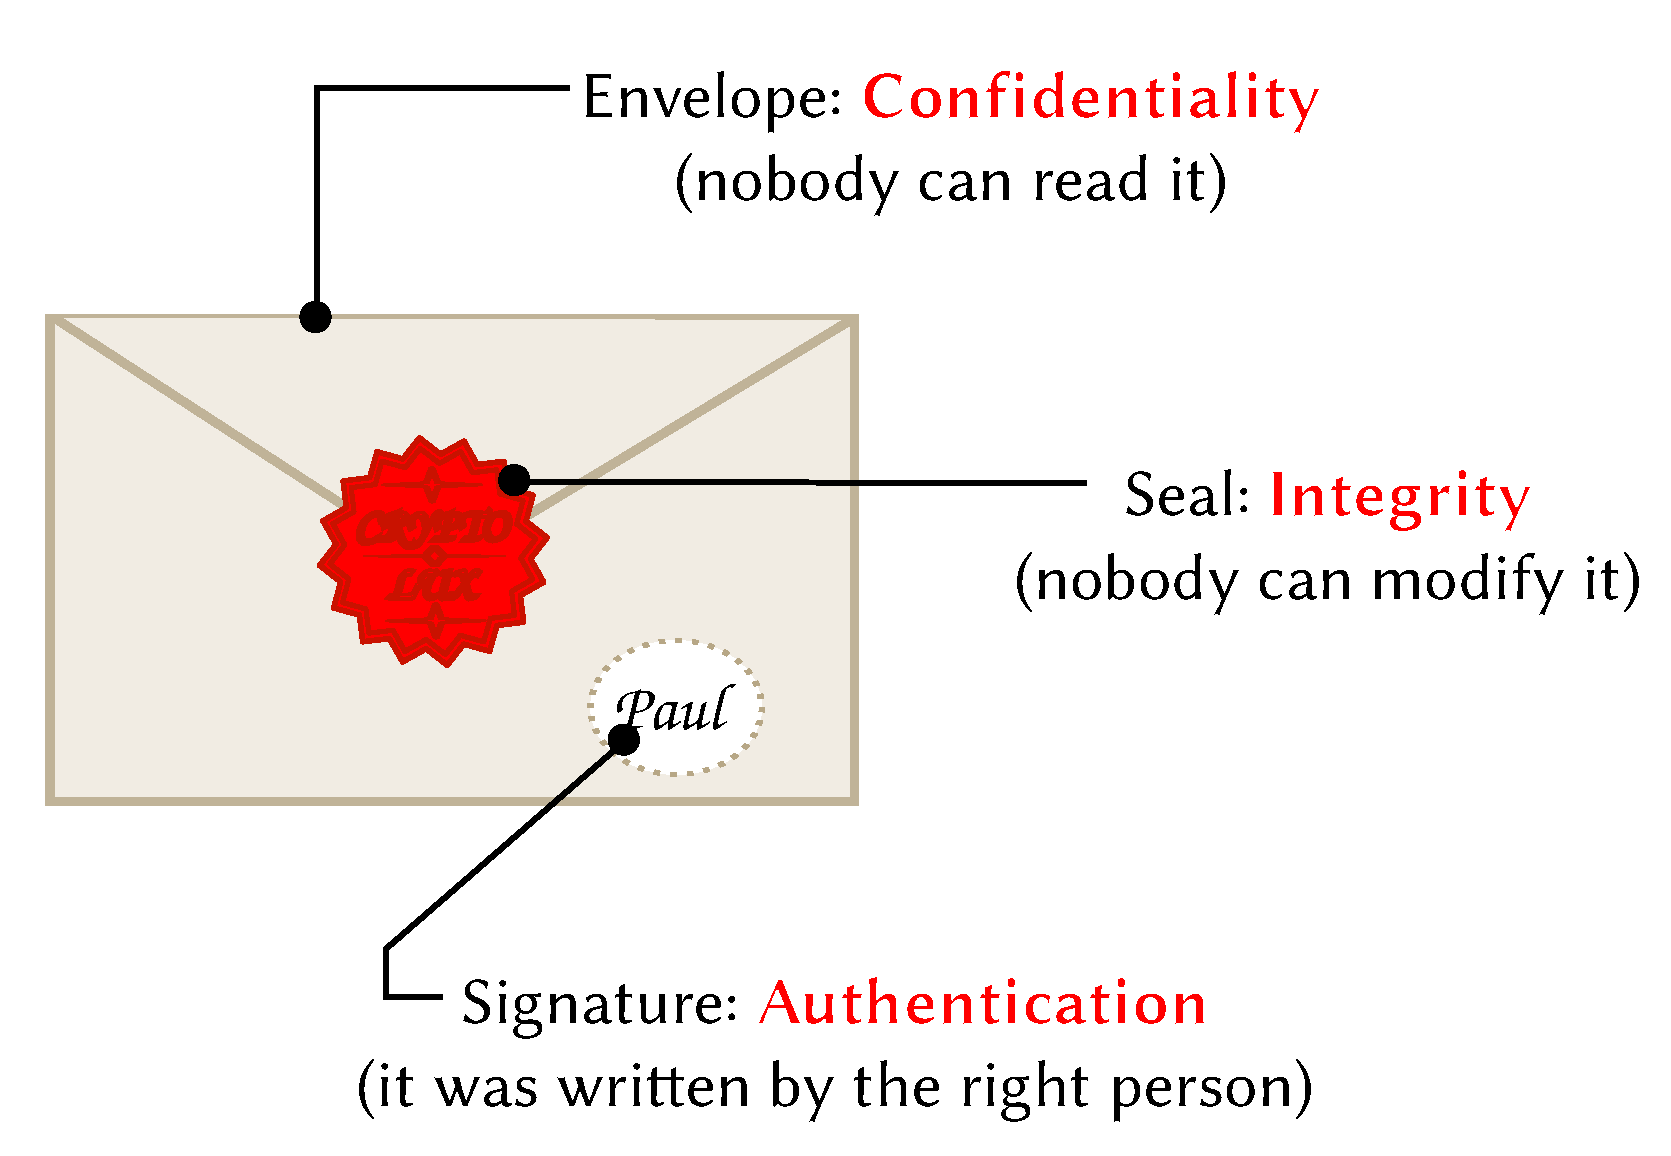
\includegraphics[width=9cm]{./figures/crypto-all}}
  \end{center}
\end{frame}


\begin{frame}{Securing Computation}
  \begin{center}
    {\Large More and more protocols intend to secure whole \alert{computations}.}

    \vspace{0.8cm}
    
    \begin{description}
    \item[FHE] \alert{F}ully \alert{H}omomorphic \alert{E}ncryption
    \item[MPC] \alert{M}ulti \alert{P}arty \alert{C}omputations
    \item[ZK-*] \alert{Z}ero \alert{K}nowledge- $[$ proof, argument... $]$
    \end{description}
  \end{center}
\end{frame}


\subsection{Different Protocols for Different Goals}

\begin{frame}{FHE}
  \begin{exampleblock}{Goal}
    Allow a third party to perform some operations on encrypted ciphertext that correspond to meaningfull operations on the corresponding plaintext. \hfill \pause \alert{A form of commutation}    
  \end{exampleblock}

  \pause

  \begin{center}
    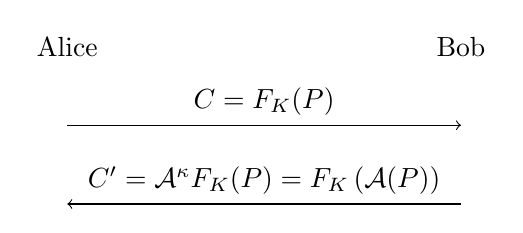
\begin{tikzpicture}
      \draw (0, 0) node(A){Alice} ;
      \draw (5, 0) node(B){Bob} ;
      \draw[->] (0, -1) -- (5, -1) node[pos=0.5,above]{$C = F_K(P)$};
      \draw[->] (5, -2) -- (0, -2) node[pos=0.5,above]{$C' = \mathcal{A}^{\kappa} F_K(P) = F_K\left(\mathcal{A}(P)\right)$};
    \end{tikzpicture}
  \end{center}

  \pause

  \begin{alertblock}{Trivial example}
    XOR-ing a constant to a ciphertext obtained using a stream cipher XORs the same constant in the plaintext.
  \end{alertblock}
\end{frame}



% !TODO! do MPC in general

\begin{frame}{Multi-Party Computations (1/2)}
  
\end{frame}

% !TODO! do masking as a particular case
\begin{frame}{Multi-Party Computations (2/2)}
  Masking
\end{frame}

% !TODO! do ZK (SNARK?) Private set intersection?


\subsection{One Approach to Rule Them All (?): Arithmetization}

\begin{frame}{Arithmetization: General Principle}
  %!TODO! write about arithmetization 
  

  \begin{center}
    \includegraphics[width=8cm]{./figures/simpsons}
  \end{center}
  
\end{frame}


\begin{frame}{``Arithmetization-Oriented''?}
  (the term was coined in~\cite{ToSC:AABDS20})
  
  \vfill

  \begin{center}
    \includegraphics[width=8cm]{./figures/simpsons}
  \end{center}
  
  \vfill

\end{frame}


\begin{frame}{Symmetric Techniques for Advanced Protocols}
  \begin{center}
    \begin{tikzpicture}[xscale=1.0, yscale=1.0]
      % Protocols
      \draw[color=dark-gray] (5, 1) node{{\Large FHE}} ; 
      \draw[color=dark-gray] (0, 1) node{{\Large MPC}} ; 
      \draw[color=dark-gray] (10, 1) node{{\Large ZK}} ;
      \pause
      % -- MPC
      \draw (0, -1) node {Masking} ;
      \draw (0, -2) node {MPC-in-the-head} ;
      \draw (0, -2.5) node {(signatures...)} ;
      \draw (0, -4) node {PCF} ;
      \draw (0, -5) node {VDF} ;
      % -- FHE
      \draw (5, -1) node {BGV} ;
      \draw (5, -2) node {BLV} ;
      \draw (5, -4) node {TFHE} ;
      % -- ZK
      \draw (10, -1) node {R1CS} ;
      \draw (10, -2) node {AIR} ;
      \draw (10, -4) node {Plonk} ;
      % AO?
      \pause
      \draw[color=navy] (-2, -3) rectangle (12, 0) ;
      \draw[color=navy,style=dotted] (8, -5) rectangle (12, -3) ;
      \draw[color=navy] (9.5, 0.2) node{Arithmetization-Oriented} ;
      \pause
      \draw[color=brown,style=dashed] (-1.9, -2.9) rectangle (6.5, -0.7) ;
      \draw[color=brown] (5.5, -0.5) node {AO evaluation};
      \pause
      \draw[color=darkgreen,style=dashed] (8.5, -4.7) rectangle (11.5, -0.7) ;
      \draw[color=darkgreen] (10.1, -0.5) node {AO verification};
      \pause
      \draw[color=pink] (-1.5, -4.4) rectangle (1.5, -3.6) ;
      \pause
      \draw[color=magenta] (3.3, -4.4) rectangle (6.7, -3.6) ;
      \pause
      \draw[color=orange] (-1.5, -5.4) rectangle (1.5, -4.6) ;
      % Alphabets
      \pause                    % masking
      \draw[color=red] (1.2, -1) node{$\mathbb{F}_2^n ; \mathbb{F}_p$} ;
      \pause                    % mpc in the head
      \draw[color=red] (1.8, -2.25) node{$\mathbb{F}_q$};
      \pause                    % PCF
      \draw[color=red] (1.2, -4) node{$\mathbb{F}_2^n$};
      \pause                    % VDF
      \draw[color=red] (1.2, -5) node{$\mathbb{F}_q$};
      \pause                    % BGV
      \draw[color=red] (5.7, -1) node{$\mathbb{F}_2^n$} ;
      \pause                    % BLV
      \draw[color=red] (5.7, -2) node{$\mathbb{F}_2^n$} ;
      \pause                    % TFHE
      \draw[color=red] (6, -4) node{$\mathbb{Z} / m \mathbb{Z}$} ;
      \pause                    % ZK
      \draw[color=red] (11, -2.5) node{$\mathbb{F}_p$};
      \onslide<1->
    \end{tikzpicture}
  \end{center}
\end{frame}


\section{Symmetric Primitives for Advanced Protocols}

\subsection{FHE: Stream ciphers for transciphering}

\begin{frame}{The case of TFHE}
  Operates on $\Zmod{\myq}$, where $\myq$ can be anything, though:
  more efficient if $\myq$ is smaller.
  
  \begin{exampleblock}{Operations allowed}
    \begin{description}
    \item[Linear Combinations] $\sum_i \myalpha_i \myx_i$, where the $\myalpha_i$ are constant while $\myx_i$ is input/key dependent.

      \begin{itemize}
      \item Costs almost nothing in terms of time/communication complexity...
      \item But \alert{noise} increases
      \end{itemize}
      \pause
    \item[PBS] (\alert{P}rogrammable \alert{B}oot\alert{S}trap) \hspace{0.5cm} $\myy \gets \myS(\myx)$
      \begin{itemize}
      \item Very time consuming...
      \item But resets the noise to a \alert{base level} \pause
      \item Can be composed with \alert{arbritrary table lookups!} \pause \hfill {\emph{\color{gray}$*$ S-box sounds $*$}}
      \item If the ring size is even, it is better if it is \alert{nega-cyclic}
      \end{itemize}
    \end{description}
  \end{exampleblock}
\end{frame}

\begin{frame}{TFHE: corresponding stream ciphers}
  \begin{description}
    \setlength\itemsep{0.3cm}
  \item[Elisabeth-4] \cite{AC:CHMS22} ; $\myq = 2^4$
    \begin{itemize}
    \item Uses a constant key register on which index-dependent non-linear functions are applied.
    \item Can be linearized~\cite{AC:GBJR23}
    \end{itemize}
    \pause
    
  \item[Gabriel...] \cite{INDOCRYPT:HofMeaSta23}  (Elisabeth-4 follow-ups)
    \pause
    
  \item[FRAST] \cite{ToSC:CCHLOS24} ; $\myq = 2^4$
    \begin{itemize}
    \item A block cipher in a CTR-mode variant.
    \item {\color{darkgreen}See you at the rump session :D}
    \end{itemize}
    \pause
    
  \item[Transistor] \cite{EPRINT:Transistor} ; $\myq = 2^4+1$
    \begin{itemize}
    \item SNOW-like round structure
    \item {\color{darkgreen}See you at Anne's invited talk :D} \pause
    \end{itemize}
  \end{description}
\end{frame}


\section{Conclusion}

\begin{frame}{Conclusion}
  \pause\vspace{1cm}
  
  \begin{center}
    \textbf{Thank you!}
  \end{center}
\end{frame}

\appendix

\bibliographystyle{alpha}
\bibliography{../abbrev2,../crypto,../biblio}


\end{document}




% Local Variables:
% compile-command: "xelatex presentation.tex"
% End:
